\documentclass[../main/git_course_main.tex]{subfiles}
\begin{document}

\setcounter{chapter}{4}
\chapter{Remote repositories}

% Removing remote branch:
% git branch -dr origin/feature-branch

\section{Overview}

In this chapter, we will go through:

\begin{itemize}
	\item Remote repositories
	\item Cloning the repository of a bioinformatic software (STAR)
	\item Merge conflicts with remote
	\item Setting up a new GitHub repository
\end{itemize}

Up until now we have been working with a single, local, instance of our
repository. This is useful by itself, but Git really starts to shine
when you start using a remote repository. By using a remote repository, you can access
your files and history from any computer and allow others to access and contribute to the code base.

Furthermore, if you are using a service such as GitHub, you are able to access your code through the web browser at any time.

\subsection{File tree / stage / repository / remote}

In this chapter, we are introducing the final layer used in Git.
Previously, we have been working with the file tree, the stage and the repository.
Hopefully, you both have a firm grasp of their different purposes now, and are feeling comfortable with the commands used for working with a local repository.

Now, we will introduce the remote repository, which simply is another copy of our
repository which mostly resides on a server-computer (for example on GitHub's servers).
We can interact with the remote to retrieve changes sent to it from other users,
and we can send our own changes to the remote. The whole process is visualized in figure \ref{fig:all_stages_visualized}.

\begin{figure}[h!]
	\centering
	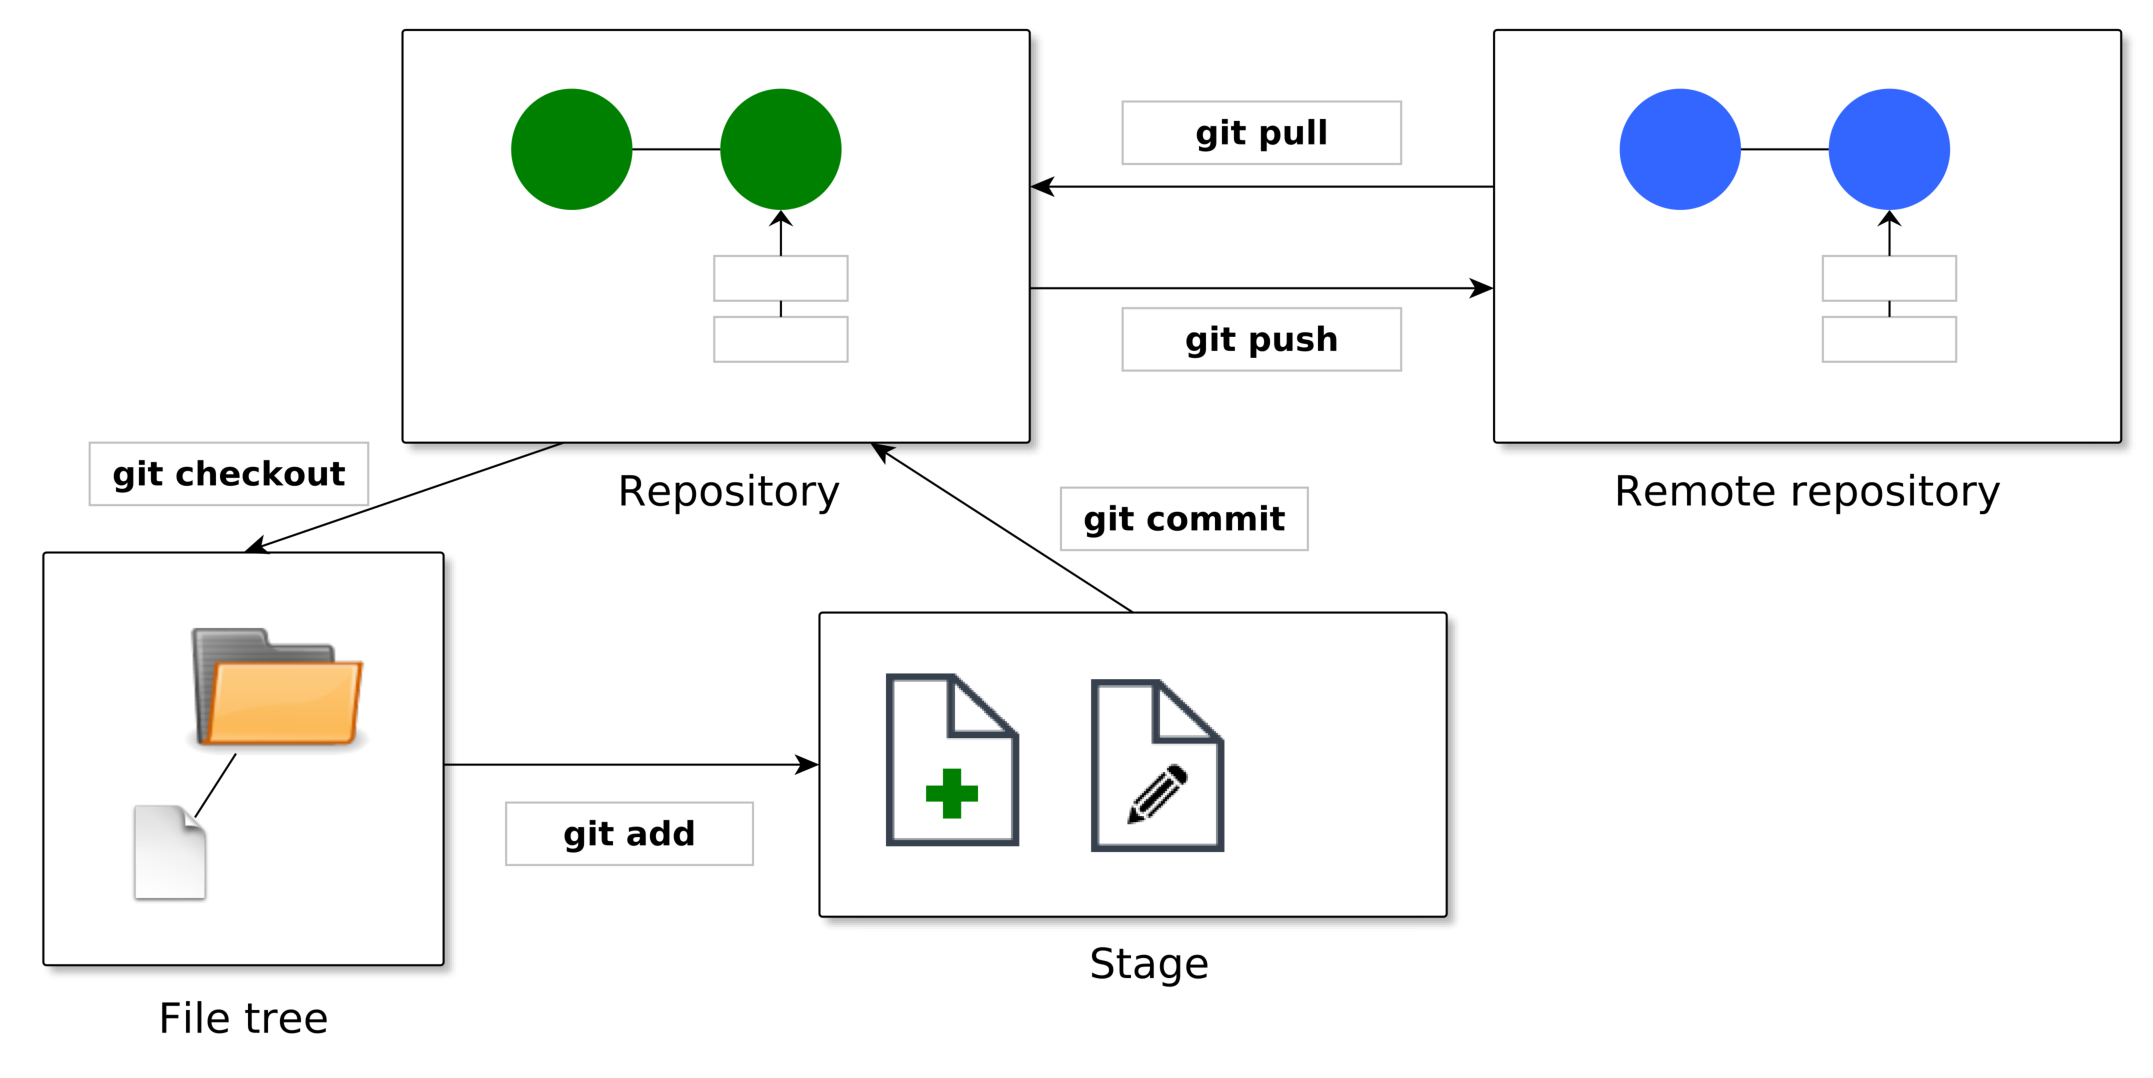
\includegraphics[width=1.0\textwidth]{../visualizations/chapter5/51_stages_including_remote.pdf}
	\caption{Visualization of the different stages in Git}
	\label{fig:all_stages_visualized}
\end{figure}

Files commonly travel the following path in Git:

\begin{enumerate}
\item They get created or added to the file tree.
\item The changes are added to the stage, prepared for being committed to history.
\item The staged set of changes gets captured into a commit, which is stored in the repository.
\item Changes made to the repository are synced with the remote repository. This means that changes made to the remote is implemented in our local repository, and changes made to our local repository is implemented into the remote.
\end{enumerate}

The remote repository is simply a regular repository which we have specified as the \verb$remote$. Commonly, many local repositories have the same remote specified and uses it as  a central point to send and retrieve changes to/from. This is visualized in Figure \ref{fig:local_remote_repos}.

\begin{figure}[h!]
	\centering
	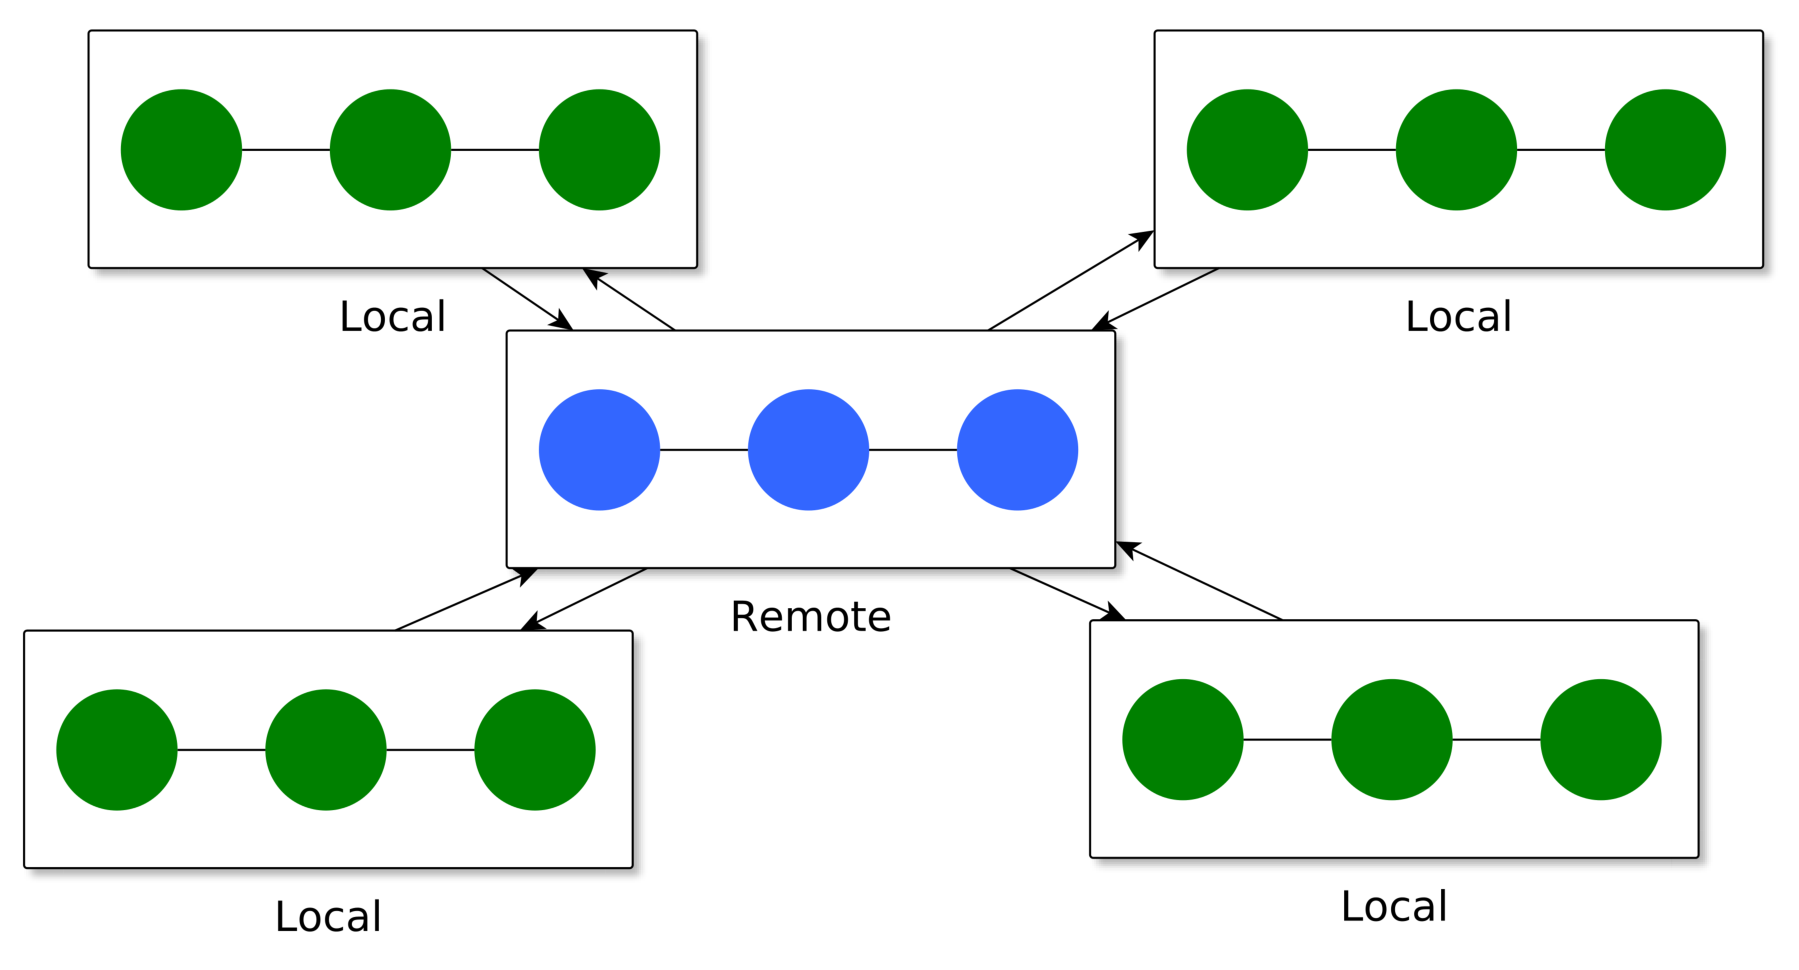
\includegraphics[width=0.8\textwidth]{../visualizations/chapter5/52_many_interacting_with_remote.pdf}
	\caption{Many local repositories are often interacting with a single remote}
	\label{fig:local_remote_repos}
\end{figure}

\section{Cloning a repository}

When you copy an existing Git repository, it is said that you \verb$clone$ that repository. 
When cloning in Git, you get a full local version of the repository which is identical
to the one you cloned. You then have access to the entire history of the repository.

Often anyone can to retrieve the entire repository, and later edits made to it,
but in general, only selected users are able to send their changes directly. In open source development something called \textit{pull requests} is used to propose edits to the remote which then can be approved or rejected by an admin.

\subsection{Cloning the STAR repository}

Many bioinformatic software is available in open repositories, often hosted on GitHub. In this chapter, we will work with the STAR repository. STAR (Spliced Transcripts Alignment to a Reference) is a popular spliced-read-aligner, similar to TopHat but with much faster processing speed (and higher RAM requirements). It is hosted on GitHub at the following address: \\

\url{https://github.com/alexdobin/STAR} \\

If you navigate to that address you will see a visual display of the source files, a README and some graphical tools which can be used to interact with and find out more about the repository. This is a Git repository similar to the one we created in the previous chapters which is hosted on GitHub's servers.

To clone the repository, we need to use its address. It is the same as the URL for the GitHub page, with an added \verb$.git$ at the end.

\begin{verbatim}
https://github.com/alexdobin/STAR.git
\end{verbatim}

To clone the repository, we run the \verb$git clone$ command, and supply the URL to the Git repository.

\begin{codebox}
\begin{lstlisting}
$ git clone https://github.com/alexdobin/STAR.git
\end{lstlisting}
\end{codebox}

%%%% GIT CLONE %%%%%
\begin{figure}[h!]
\begin{bluebox}
Command: \verb$git clone <path>$ \\

Create a full local copy of the target Git-repository.
\end{bluebox}
\label{command:clone}
\caption{git clone - Create a local copy of a repository}
\end{figure}
%%%%%%%%%%%%%%%%%%%%%%

This will create a folder in your current working directory, which will contain the repository. We can now navigate into the repository and take a look. We will investigate it further in the exercises.

\section{Clone and work with an existing repository}

In the previous section, we created a copy of the STAR repository. The version hosted
on GitHub is the \verb$remote$ repository for STAR. After cloning we have an exact local
copy of it. The only thing distinguishing the remote is in this case that the developers
have agreed on using the GitHub-version as their remote. Otherwise, there is nothing
special with it.

If we have the access rights (for example if we are the original author of the repository) we can make changes to the remote by first making local changes, and then pushing them to the remote location.

\subsection{Cloning the remote}

Here, we will do a brief demonstration of how it could look if you had access rights
to a particular repository and wanted to make changes after cloning it. Note - 
You do not have access to the particular repository used in this example, which means that you cannot push changes to it.

\begin{codebox}
\begin{lstlisting}
$ git clone https://github.com/Jakob37/GitCourse.git
Cloning into 'GitCourse'...
remote: Counting objects: 15, done.
remote: Total 15 (delta 0), reused 0 (delta 0), pack-reused 15
Unpacking objects: 100% (15/15), done.
Checking connectivity... done.
$ cd GitCourse
$ git log --oneline
ff79a43 Add files
c43f754 First commit
\end{lstlisting}
\end{codebox}

At this point, we have cloned the remote repository which contains two commits. Now, we have a local copy of it.
Figure \ref{fig:original_state} shows how the repository looks before making any changes. Our repository contains two commits, and is synced with the remote.

\begin{figure}[h!]
	\centering
	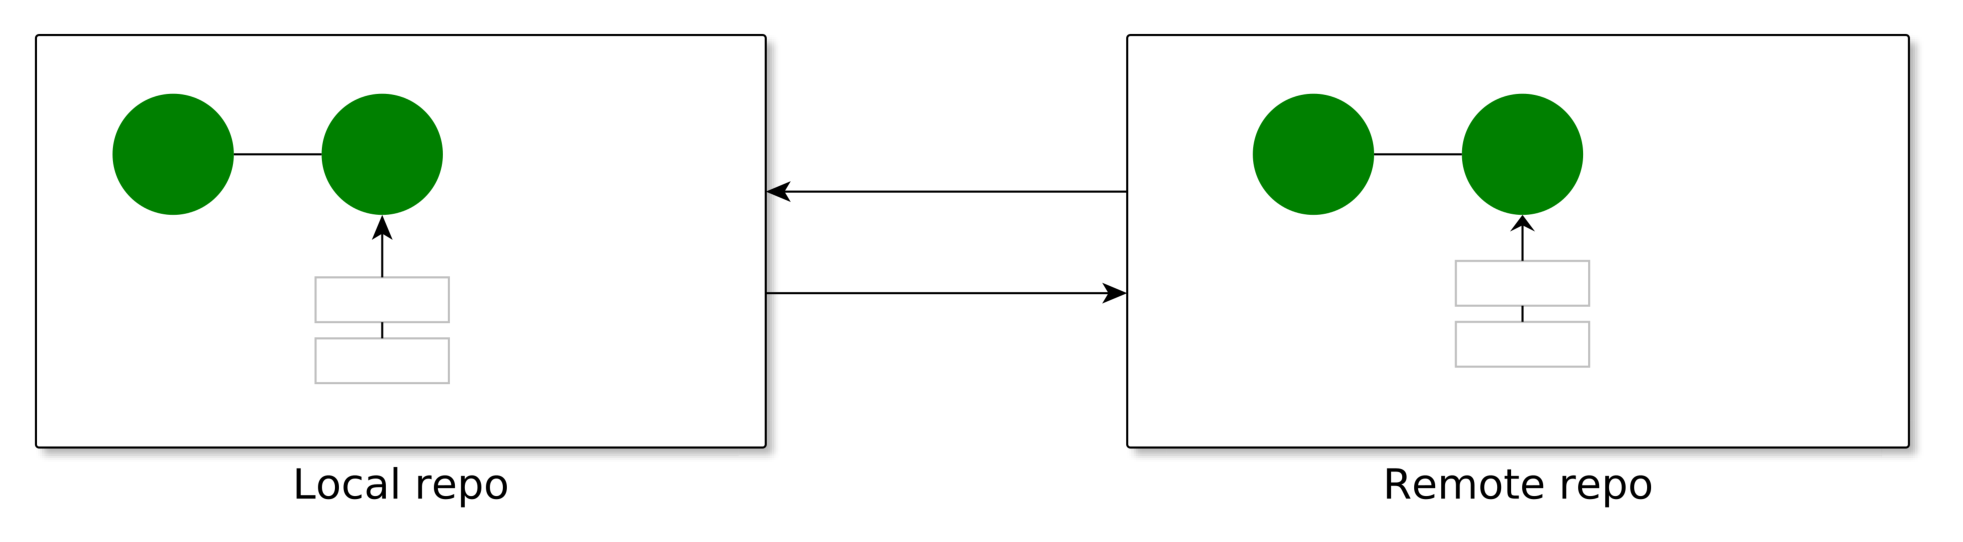
\includegraphics[width=0.8\textwidth]{../visualizations/chapter5/530_local_remote_synced.pdf}
	\caption{State of the local and remote repositories - No local changes}
	\label{fig:original_state}
\end{figure}

\subsection{Making local changes}

\begin{codebox}
\begin{lstlisting}
$ nano ruby_hi.rb
$ cat ruby_hi.rb
#!/usr/bin/ruby
print("HI!\n")
$ git add ruby_hi.rb
$ git commit -m "Add Ruby Hi script"
\end{lstlisting}
\end{codebox}

Now, we added a small Ruby script printing "HI!". We also staged the file for being committed, and finally created a commit.

The current state of the repository is shown in figure \ref{fig:local_changes}. The purple commit is the newly created local commit. As we haven't sent the commit to the remote, our remote only contains the two first commits.

\begin{figure}[h!]
	\centering
	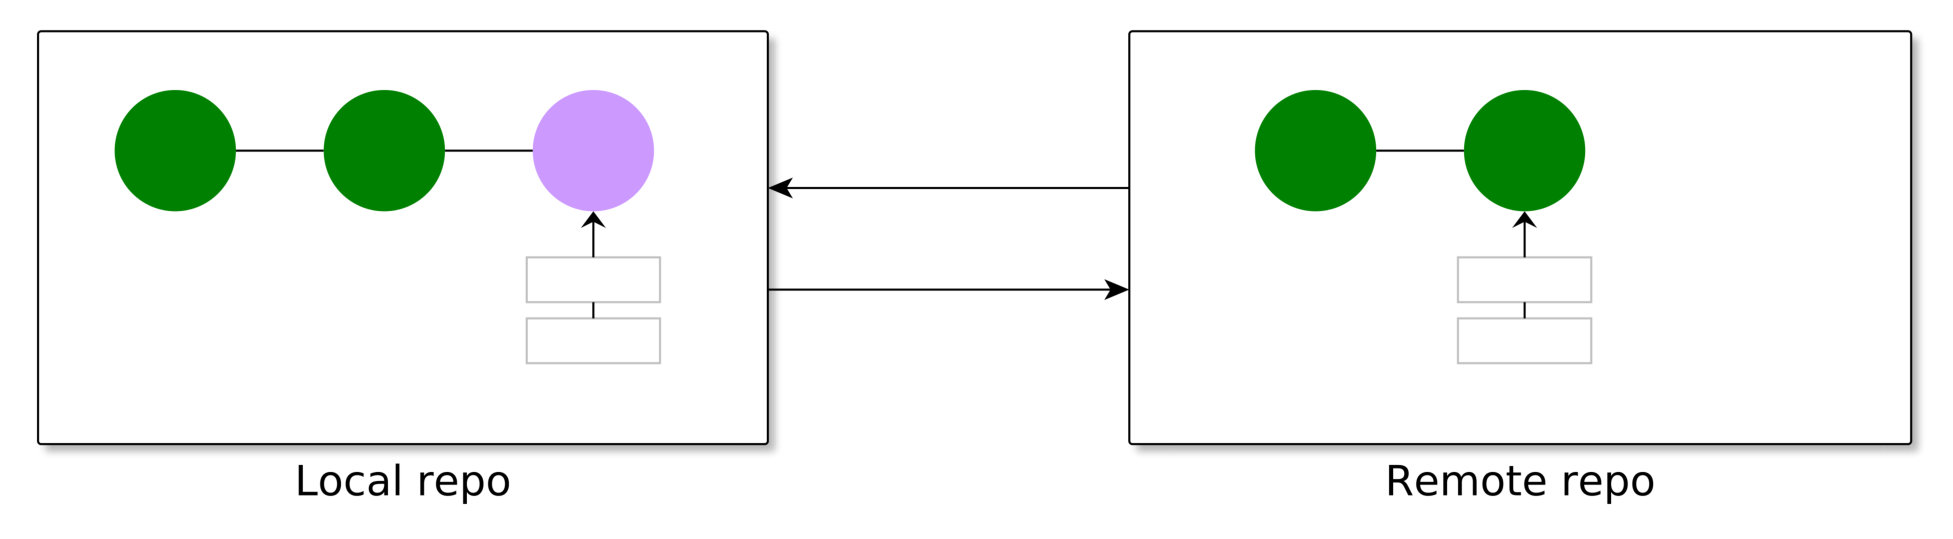
\includegraphics[width=0.8\textwidth]{../visualizations/chapter5/53_local_changes_made.pdf}
	\caption{Stage of the repo, local and remote - Local changes pushed to remote}
	\label{fig:local_changes}
\end{figure}

The changes are only present locally. If others should be able to see the changes, we need to send them to the remote too.
The repository pushes per default the repository to a head called \verb$origin$. To see the current remote paths for pulling and pushing, we can use the command \verb$git remote -v$.

\begin{codebox}
\begin{lstlisting}
$ git remote -v
origin	https://github.com/Jakob37/GitCourse.git (fetch)
origin	https://github.com/Jakob37/GitCourse.git (push)
\end{lstlisting}
\end{codebox}

It looks fine here - our remote was set up properly when cloning the repository.
When creating our own remote we will need to set this up for ourselves.

%%%% GIT REMOTE %%%%%
\begin{figure}[h!]
\begin{bluebox}
Command: \verb$git remote [-v]$ \\

Get the current remote for the repository. If used with the \verb$-v$ flag,
the full URL is printed.
\end{bluebox}
\label{command:clone}
\caption{git clone - Create a local copy of a repository}
\end{figure}
%%%%%%%%%%%%%%%%%%%%%%

\subsection{Pushing to the remote}

Before pushing new commits, we want to retrieve existing changes made to the remote.

We have two commands for this. \verb$git fetch$ fetches information about changes done on the remote - but doesn't retrieve them.
\verb$git pull$ retrieves the changes from the remote, inserting the new commits into our local repository.

\begin{codebox}
\begin{lstlisting}
$ git fetch
# No output - no new changes
$ git pull
Already up-to-date.
\end{lstlisting}
\end{codebox}

%%%% GIT FETCH %%%%%
\begin{figure}
\begin{bluebox}
Command: \verb$git fetch$ \\

Update information about state of the remote.
\end{bluebox}
\label{command:fetch}
\caption{git fetch - Sync with the remote}
\end{figure}
%%%%%%%%%%%%%%%%%%%%%%

%%%% GIT PULL %%%%%
\begin{figure}
\begin{bluebox}
Command: \verb$git pull$ \\

Retrieve changes made to the remote
\end{bluebox}
\label{command:pull}
\caption{git pull - Retrieve changes made to the remote}
\end{figure}
%%%%%%%%%%%%%%%%%%%%%%

In this case, there weren't any new changes. We are free to push our new commits to the repository, so that all collaborators can access them. Note: This is only possible to do if you have access to the repository.

\begin{codebox}
\begin{lstlisting}
$ git push
# You are prompted for username and password
Username for 'https://github.com': Jakob37
Password for 'https://Jakob37@github.com': 
Counting objects: 7, done.
Delta compression using up to 8 threads.
Compressing objects: 100% (5/5), done.
Writing objects: 100% (5/5), 614 bytes | 0 bytes/s, done.
Total 5 (delta 1), reused 0 (delta 0)
To https://github.com/Jakob37/GitCourse.git
   984f0ac..3ab3714  master -> master
\end{lstlisting}
\end{codebox}

When pushing changes, you are prompted for your username and password.
Figure \ref{fig:changes_pushed} shows the state of the local and remote repositories after pushing the changes.

\begin{figure}[h!]
	\centering
	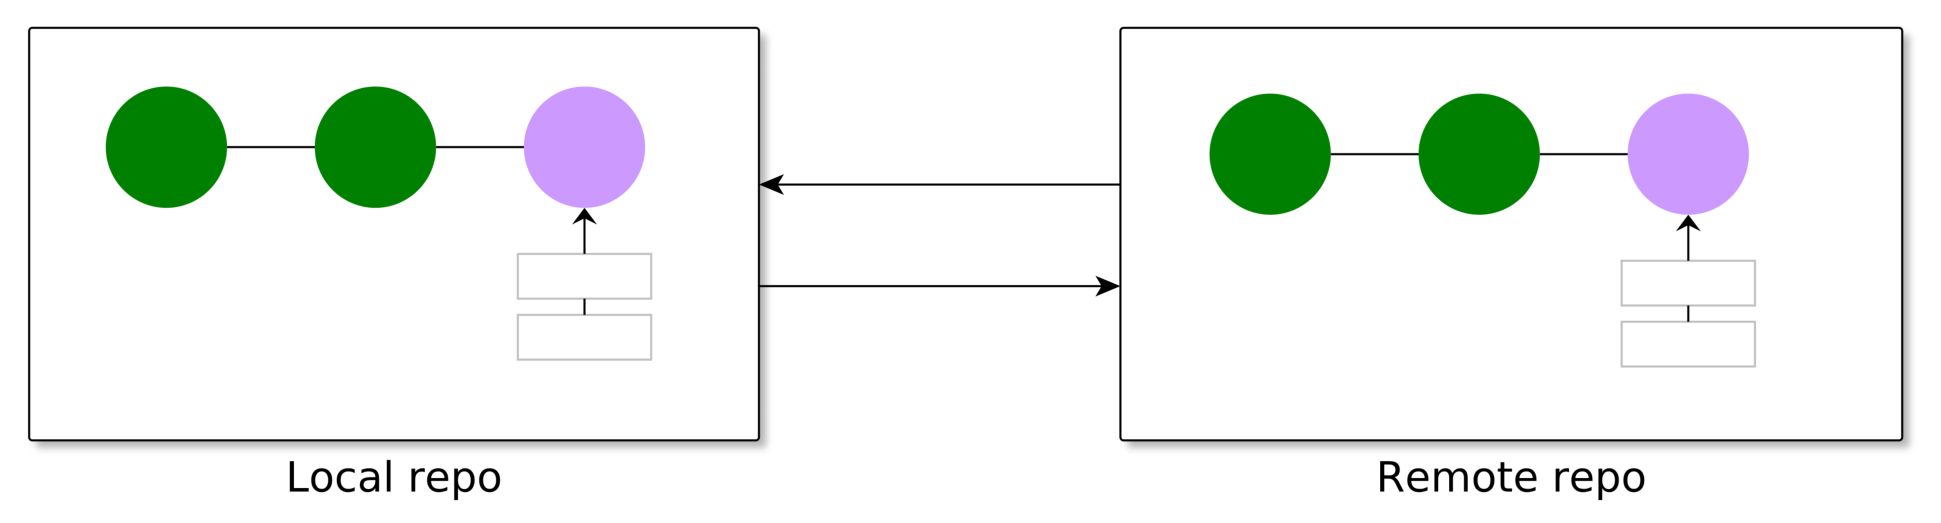
\includegraphics[width=0.8\textwidth]{../visualizations/chapter5/54_changes_pushed.pdf}
	\caption{Stage of the repo - Local changes pushed to the remote}
	\label{fig:changes_pushed}
\end{figure}

%%%% GIT PUSH %%%%%
\begin{figure}
\begin{bluebox}
Command: \verb$git push$ \\

Send local commits to the remote
\end{bluebox}
\label{command:pull}
\caption{git push - Send local commits to the remote}
\end{figure}
%%%%%%%%%%%%%%%%%%%%%%

\section{Parallel changes to the local and to the remote}

Let's back up to before pushing our changes to the remote and investigate how it would look if there would have been changes made to the remote. If there already were changes made to the remote, we would get the following output from the \verb$git fetch$ command:

\begin{codebox}
\begin{lstlisting}
$ git fetch
remote: Counting objects: 3, done.
remote: Compressing objects: 100% (2/2), done.
remote: Total 3 (delta 0), reused 3 (delta 0), pack-reused 0
Unpacking objects: 100% (3/3), done.
From https://github.com/Jakob37/GitCourse
   a75107d..984f0ac  master     -> origin/master
\end{lstlisting}
\end{codebox}

Looks like we have changes to to take into account. We can check the current status of our local master-branch compared to the \verb$origin$ by running \verb$git status$

\begin{codebox}
\begin{lstlisting}
$ git status
On branch master
Your branch and 'origin/master' have diverged,
and have 1 and 1 different commit each, respectively.
  (use "git pull" to merge the remote branch into yours)

nothing to commit, working directory clean
\end{lstlisting}
\end{codebox}

Figure \ref{fig:diverged_remote} shows the current state of the repositories.

\begin{figure}[h!]
	\centering
	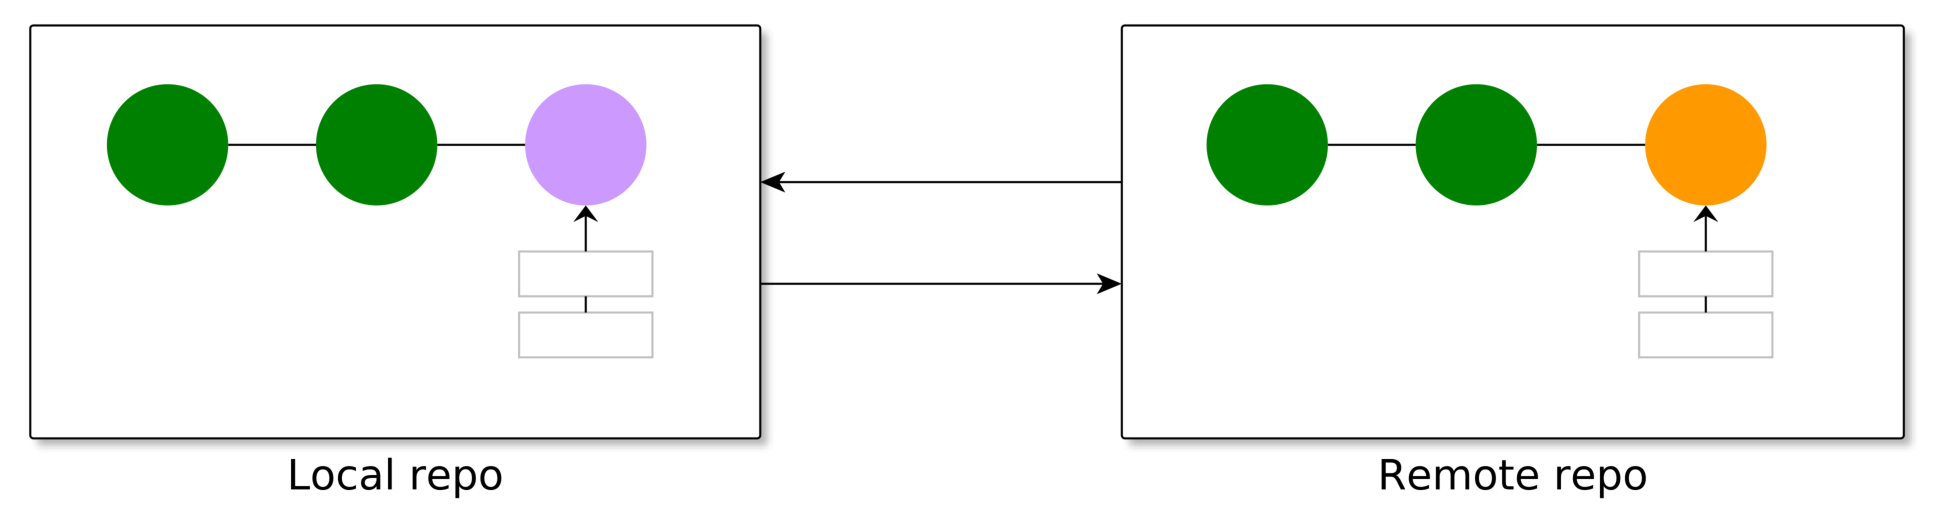
\includegraphics[width=1.0\textwidth]{../visualizations/chapter5/55_diverging_commits.pdf}
	\caption{Diverging commits on master and remote}
	\label{fig:diverged_remote}
\end{figure}

If we try to push at this point we will get prompted for username and password, and then
get the following message:

\begin{codebox}
\begin{lstlisting}
$ git push
Username for 'https://github.com': Jakob37
Password for 'https://Jakob37@github.com': 
To https://github.com/Jakob37/GitCourse.git
 ! [rejected]        master -> master (non-fast-forward)
error: failed to push some refs to 
'https://github.com/Jakob37/GitCourse.git'
hint: Updates were rejected because the tip of your current 
hint: branch is behind its remote counterpart. Integrate the 
hint: remote changes (e.g. 'git pull ...') before pushing 
hint: again. See the 'Note about fast-forwards' in 
hint: 'git push --help' for details.
\end{lstlisting}
\end{codebox}

We need to retrieve and integrate the remote edits in our repository before pushing
our changes to the remote.

To do this, we will create a merge commit (similarly to when we were working with branches). If we are lucky, there are no conflicts with the remote changes.

\begin{codebox}
\begin{lstlisting}
$ git pull
# Here, the default text editor is opened
# Enter commit message, and then save/quit
 perl_hi.pl | 3 +++
 1 file changed, 3 insertions(+)
 create mode 100644 perl_hi.pl
\end{lstlisting}
\end{codebox}

It seems like there were no conflicts. If there are, those are managed similarly to what was shown for branches in the previous chapter. The state of the local and remote repositories is shown in figure \ref{fig:integrated_remote_changes}. We have both the local and the remote edits, as well as a merge commit.

We are ready to push our edits.

\begin{figure}[h!]
	\centering
	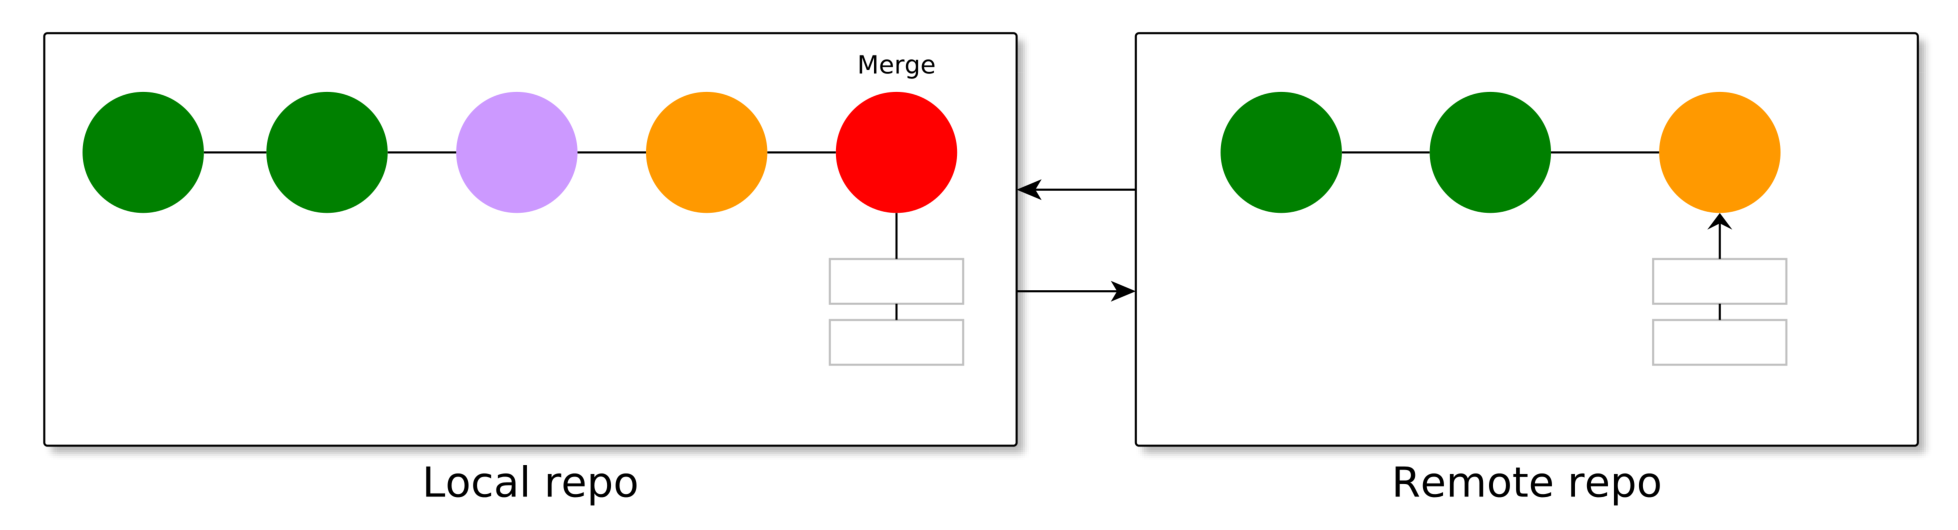
\includegraphics[width=1.0\textwidth]{../visualizations/chapter5/56_integrating_remote_changes.pdf}
	\caption{Integrating remote changes}
	\label{fig:integrated_remote_changes}
\end{figure}

\begin{codebox}
\begin{lstlisting}
$ git push
Username for 'https://github.com': Jakob37
Password for 'https://Jakob37@github.com': 
Counting objects: 7, done.
Delta compression using up to 8 threads.
Compressing objects: 100% (5/5), done.
Writing objects: 100% (5/5), 614 bytes | 0 bytes/s, done.
Total 5 (delta 1), reused 0 (delta 0)
To https://github.com/Jakob37/GitCourse.git
   984f0ac..3ab3714  master -> master
\end{lstlisting}
\end{codebox}

Now, the remote has finally received our changes. The final state of the repositories is shown in figure \ref{fig:pushing_merged_commits}:

\begin{figure}[h!]
	\centering
	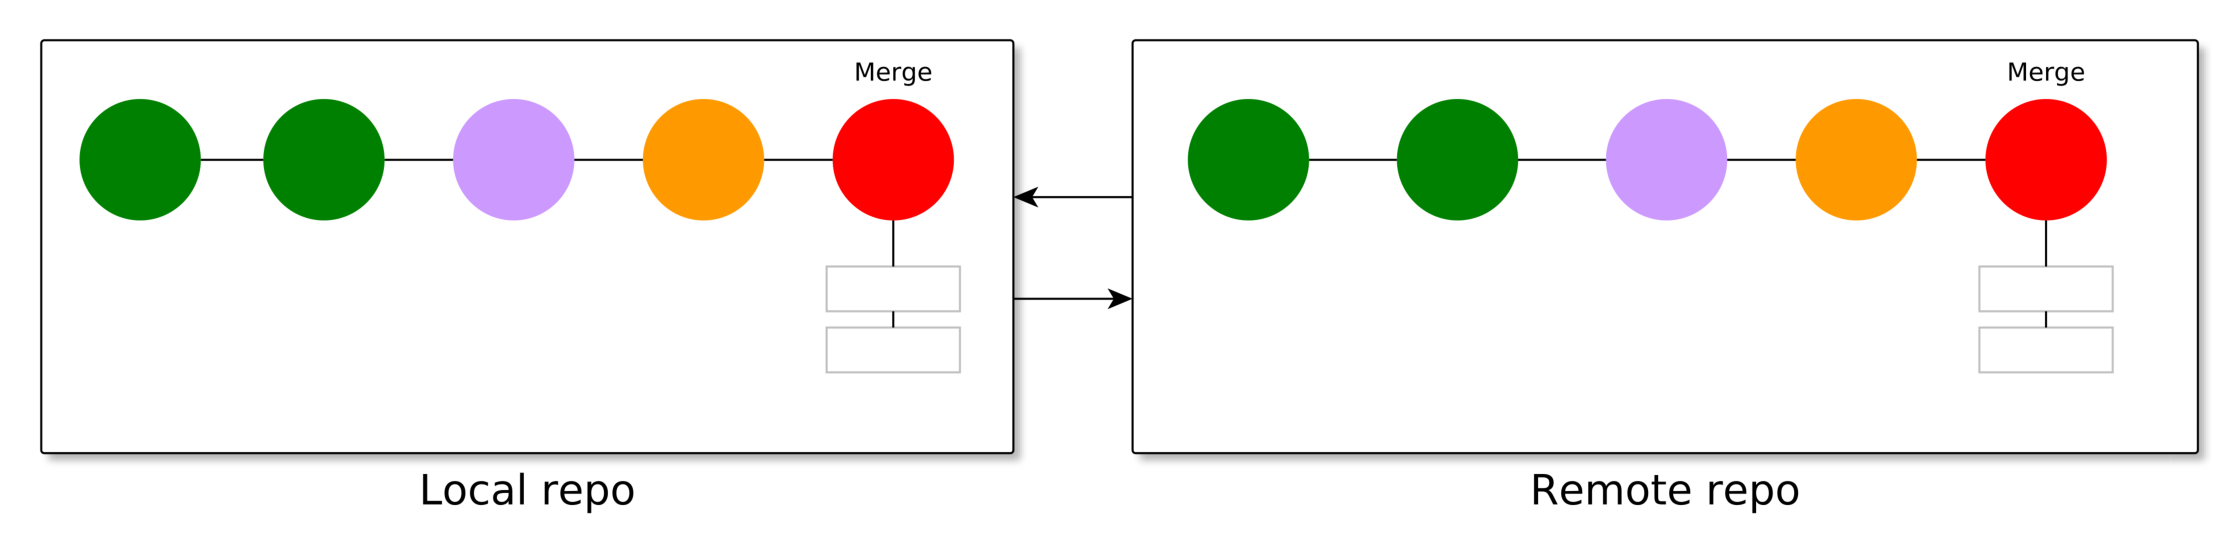
\includegraphics[width=1.0\textwidth]{../visualizations/chapter5/57_pushing_merged_commits.pdf}
	\caption{Final state after pushing merged changes}
	\label{fig:pushing_merged_commits}
\end{figure}

\section{Setting up a remote on GitHub}

Now, let's see how we can set up a remote repository for a local repository which we already have been working with.
In this case, we will go though how to set it up on GitHub. If using other services, the way of creating the remote will be slightly different.

To use GitHub, we first need to create a new account. After going through the usual steps, we are ready to start creating a new repository by clicking "Create repository".

Here, we can fill in some information about the remote. The absolute minimum is a name for our newly created GitHub repo. This is shown in figure \ref{fig:github_repo_details}

\begin{figure}[h!]
	\centering
	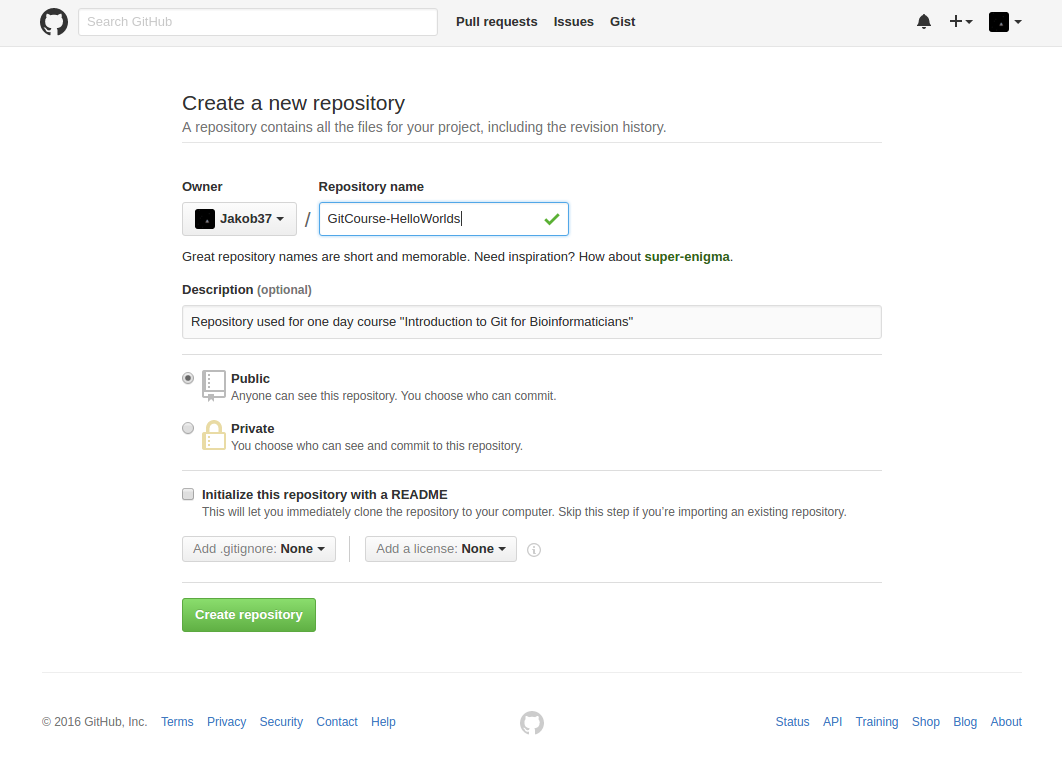
\includegraphics[width=1.0\textwidth]{../visualizations/screenshots/git_course_hello_worlds_repo.png}
	\caption{Details for the new repository}
	\label{fig:github_repo_details}
\end{figure}

Now, let's initiate a local repository for which we want to assign our remote.

\begin{codebox}
\begin{lstlisting}
$ git init
$ touch a_file.txt
$ git add a_file.txt
$ git commit -m "First commit"
\end{lstlisting}
\end{codebox}

We are now ready to assign this as the remote for our local repository. To do this,
we need to first use the \verb$git remote add$ command to set up the repository as our new remote. Then, initiate using this remote by using the \verb$--set-upstream$ flag with the \verb$git push$ command.

Finally, check that you have assigned the correct URLs using the \verb$git remote -v$ command.

\begin{codebox}
\begin{lstlisting}
$ git remote add origin https://github.com/Jakob37/GitCourse.git
$ git push --set-upstream origin master
Username for 'https://github.com': Jakob37
Password for 'https://Jakob37@github.com': 
Counting objects: 3, done.
Delta compression using up to 8 threads.
Compressing objects: 100% (2/2), done.
Writing objects: 100% (3/3), 221 bytes | 0 bytes/s, done.
Total 3 (delta 0), reused 0 (delta 0)
To https://github.com/Jakob37/testtesttest.git
 * [new branch]      master -> master
Branch master set up to track remote branch master from origin.
$ git remote -v
origin https://github.com/Jakob37/GitCourse.git (fetch)
origin https://github.com/Jakob37/GitCourse.git (push)
\end{lstlisting}
\end{codebox}

We are now ready to push and pull similarly to how we did before.
If you get error messages, double-check that you have the correct paths.

%%%% GIT REMOTE %%%%%
\begin{figure}[h!]
\begin{bluebox}
Command: \verb$git remote add origin <path>$ \\
Command: \verb$git push --set-upstream origin master$ \\
Command: \verb$git remote -v$ \\

Collection of commands used to set up the link to the remote properly,
and to check that the URLs are correct.
\end{bluebox}
\label{command:pull}
\caption{Commands for setting up the remote}
\end{figure}
%%%%%%%%%%%%%%%%%%%%%%

\section{GitHub, Bitbucket, and other places to host your repo}

You can set up a remote on your own server (if you have access to one), but there are also
a lot of great services available for hosting. Two of the most popular services are GitHub and Bitbucket, which both provides a graphical interface with a lot of functionality for working with the remote.

\subsection{GitHub}

\url{https://github.com} \\

GitHub is perhaps the most widely used hosting service for Git repositories, and is frequently used for hosting of open source bioinformatics software. 

GitHub allows hosting of an unlimited number of both public and private repositories for free, with an unlimited number of collaborators to boot. If you pay a monthly subscription, you get access to benefits like increased storage space and support. In the past, all users were limited to a maximum of five repositories, regardless of subscription.

\subsection{Bitbucket}

\url{https://bitbucket.org} \\

Bitbucket is another popular hosting service provided by the software group Atlassin. It used to have an edge over GitHub in that it supported Mercurial in addition to Git, but that is no longer the case. The perhaps most relevant difference now is the payment model. As a Bitbucket subscriber, you pay for the number of collaborators (people with edit rights to the repositories). If you want to have more than five contributors to a repository, you must pay up. As is true for GitHub, paying users also get other benefits like storage space and other features.

\newpage
\section{Exercises}

\subsection{Working with remote GitHub repositories}

\begin{enumerate}

\item Go to \url{github.com} and create a new account.
\item Create a new repository on GitHub by clicking "New repository" (Green button). Give it a name, and make sure to pick the "Public" option.
\item Set up this as a remote for the repository you have been building throughout this course.
\item Push your repository, and check on GitHub that you can see all of your files and commits in the interface.
\end{enumerate}

\subsection{Collaborating with classmates on GitHub repositories (*)}

Do this exercise if you have the time. If you are in a hurry, come back to this exercise after reading through the final chapter.

\begin{enumerate}
\item Give a friend with a GitHub account access to your repository (and make sure that you get access in return).
\item Clone your friends repository. Investigate the files, and the log. Have your friend been using clear commit messages?
\item Contribute to your friends repository by creating a new file, or making (reasonable) edits to one of his or her files.
\item Push the changes to the remote.
\item Retrieve the changes which your friend have made to your repository. You can investigate the changes made in the commit by clicking "commits" and the commit(s) created by your friend.
\item As a challenge: Create commits editing the same files as the ones your friend have pushed to the remote. Solve the merge conflict that arises when you attempt to sync your changes with the repository.
\end{enumerate}

\newpage
\section{Recap}

\subsection{Concepts}

\begin{itemize}
	\item What is a remote repository, and how is it useful?
	\item What are the benefits of using a hosting-service like GitHub and Bitbucket? (And why do you think GitHub is so popular for hosting bioinformatic software)
	\item When do you encounter merge-conflicts when working with remotes?
\end{itemize}

\subsection{Commands}

\begin{itemize}
	\item \verb$git clone <path>$
	\item \verb$git fetch$
	\item \verb$git pull$
	\item \verb$git push [--set-upstream origin master]$
	\item \verb$git remote add origin <path>$
	\item \verb$git remote -v$
\end{itemize}

\end{document}
